%% ----------------------------------------------------------------
%% Thesis.tex -- MAIN FILE (the one that you compile with LaTeX)
%% ---------------------------------------------------------------- 

% Set up the document
\documentclass[a4paper, 12pt, oneside]{Thesis}  % Use the "Thesis" style, based on the ECS Thesis style by Steve Gunn
%\usepackage{caption}
%\usepackage{subcaption}
%\usepackage{subfig}
%\newsubloat{figure}
%\let\subcaption\relax
%\let\subfloat\relax
\usepackage{float}

%\let\subfigure\relax
\usepackage[turkish]{babel}
\usepackage[utf8]{inputenc}
%\thispagestyle{plain}
%\usepackage{amsmath}
%\usepackage{hyperref}
%\numberwithin{equation}{subsection}
\usepackage{graphicx}
%\usepackage{changepage}
%\usepackage[export]{adjustbox}
\usepackage{pdfpages}

%\graphicspath{Figures/}  % Location of the graphics files (set up for graphics to be in PDF format)

% Include any extra LaTeX packages required
\usepackage[square, numbers, comma, sort&compress]{natbib}  % Use the "Natbib" style for the references in the Bibliography
\usepackage{verbatim}  % Needed for the "comment" environment to make LaTeX comments
\usepackage{vector}  % Allows "\bvec{}" and "\buvec{}" for "blackboard" style bold vectors in maths
\hypersetup{urlcolor=blue, colorlinks=true}  % Colours hyperlinks in blue, but this can be distracting if there are many links.


\usepackage{etoolbox}
\let\oldincludegraphics\includegraphics
\renewcommand{\includegraphics}[2][]{%
  \oldincludegraphics[#1]{#2}%
  \shorthandon{=}%
  }
\pretocmd{\includegraphics}{\shorthandoff{=}}{}{}

\graphicspath{ {images/} }
%\usepackage{mathtools}

%\usepackage{graphicx,changepage}
%\newcommand{\adjustimg}{% Horizontal adjustment of image
%  \checkoddpage%
 % \ifoddpage\hspace*{\dimexpr\evensidemargin-\oddsidemargin}\else\hspace*{-\dimexpr\evensidemargin-\oddsidemargin}\fi%
%}
%\newcommand{\centerimg}[2][width=\textwidth]{% Center an image
 % \makebox[\textwidth]{\adjustimg\includegraphics[#1]{#2}}%
%}
%\usepackage[demo]{graphicx}
%\usepackage{subfig}
%\usepackage{wrapfig}
%\usepackage{lipsum}

%\usepackage{subfig}

%\usepackage[demo]{graphicx} %graphic side by side
%\usepackage{caption}
%\usepackage{subcaption}
%% ----------------------------------------------------------------
\begin{document}
\frontmatter      % Begin Roman style (i, ii, iii, iv...) page numbering

% Set up the Title Page
\title  {Thesis Title}
\authors  {\texorpdfstring
            {\href{your web site or email address}{Author Name}}
            {Author Name}
            }
\addresses  {\groupname\\\deptname\\\univname}  % Do not change this here, instead these must be set in the "Thesis.cls" file, please look through it instead
\date       {\today}
\subject    {}
\keywords   {}

\maketitle
%% ----------------------------------------------------------------

\setstretch{1.3}  % It is better to have smaller font and larger line spacing than the other way round

% Define the page headers using the FancyHdr package and set up for one-sided printing
\fancyhead{}  % Clears all page headers and footers
\rhead{\thepage}  % Sets the right side header to show the page number
\lhead{}  % Clears the left side page header

\pagestyle{fancy}  % Finally, use the "fancy" page style to implement the FancyHdr headers

%% ----------------------------------------------------------------
% Declaration Page required for the Thesis, your institution may give you a different text to place here
\Declaration{

\addtocontents{toc}{\vspace{1em}}  % Add a gap in the Contents, for aesthetics

I, AUTHOR NAME, declare that this thesis titled, `THESIS TITLE' and the work presented in it are my own. I confirm that:

\begin{itemize} 
\item[\tiny{$\blacksquare$}] This work was done wholly or mainly while in candidature for a research degree at this University.
 
\item[\tiny{$\blacksquare$}] Where any part of this thesis has previously been submitted for a degree or any other qualification at this University or any other institution, this has been clearly stated.
 
\item[\tiny{$\blacksquare$}] Where I have consulted the published work of others, this is always clearly attributed.
 
\item[\tiny{$\blacksquare$}] Where I have quoted from the work of others, the source is always given. With the exception of such quotations, this thesis is entirely my own work.
 
\item[\tiny{$\blacksquare$}] I have acknowledged all main sources of help.
 
\item[\tiny{$\blacksquare$}] Where the thesis is based on work done by myself jointly with others, I have made clear exactly what was done by others and what I have contributed myself.
\\
\end{itemize}
 
 
Signed:\\
\rule[1em]{25em}{0.5pt}  % This prints a line for the signature
 
Date:\\
\rule[1em]{25em}{0.5pt}  % This prints a line to write the date
}
\clearpage  % Declaration ended, now start a new page

%% ----------------------------------------------------------------
% The "Funny Quote Page"
\pagestyle{empty}  % No headers or footers for the following pages

\null\vfill
% Now comes the "Funny Quote", written in italics
\textit{``Write a funny quote here.''}

\begin{flushright}
If the quote is taken from someone, their name goes here
\end{flushright}

\vfill\vfill\vfill\vfill\vfill\vfill\null
\clearpage  % Funny Quote page ended, start a new page
%% ----------------------------------------------------------------

% The Abstract Page
\addtotoc{Abstract}  % Add the "Abstract" page entry to the Contents
\abstract{
\addtocontents{toc}{\vspace{1em}}  % Add a gap in the Contents, for aesthetics

The Thesis Abstract is written here (and usually kept to just this page). The page is kept centered vertically so can expand into the blank space above the title too\ldots

}

\clearpage  % Abstract ended, start a new page
%% ----------------------------------------------------------------

\setstretch{1.3}  % Reset the line-spacing to 1.3 for body text (if it has changed)

% The Acknowledgements page, for thanking everyone
\acknowledgements{
\addtocontents{toc}{\vspace{1em}}  % Add a gap in the Contents, for aesthetics

The acknowledgements and the people to thank go here, don't forget to include your project advisor\ldots

}
\clearpage  % End of the Acknowledgements
%% ----------------------------------------------------------------

\pagestyle{fancy}  %The page style headers have been "empty" all this time, now use the "fancy" headers as defined before to bring them back


%% ----------------------------------------------------------------
\lhead{\emph{Contents}}  % Set the left side page header to "Contents"
\tableofcontents  % Write out the Table of Contents

%% ----------------------------------------------------------------
\lhead{\emph{List of Figures}}  % Set the left side page header to "List if Figures"
\listoffigures  % Write out the List of Figures

%% ----------------------------------------------------------------
\lhead{\emph{List of Tables}}  % Set the left side page header to "List of Tables"
\listoftables  % Write out the List of Tables

%% ----------------------------------------------------------------
\setstretch{1.5}  % Set the line spacing to 1.5, this makes the following tables easier to read
\clearpage  % Start a new page
\lhead{\emph{Abbreviations}}  % Set the left side page header to "Abbreviations"
\listofsymbols{ll}  % Include a list of Abbreviations (a table of two columns)
{
% \textbf{Acronym} & \textbf{W}hat (it) \textbf{S}tands \textbf{F}or \\
\textbf{LAH} & \textbf{L}ist \textbf{A}bbreviations \textbf{H}ere \\

}

%% ----------------------------------------------------------------
\clearpage  % Start a new page
\lhead{\emph{Physical Constants}}  % Set the left side page header to "Physical Constants"
\listofconstants{lrcl}  % Include a list of Physical Constants (a four column table)
{
% Constant Name & Symbol & = & Constant Value (with units) \\
Speed of Light & $c$ & $=$ & $2.997\ 924\ 58\times10^{8}\ \mbox{ms}^{-\mbox{s}}$ (exact)\\

}

%% ----------------------------------------------------------------
\clearpage  %Start a new page
\lhead{\emph{Symbols}}  % Set the left side page header to "Symbols"
\listofnomenclature{lll}  % Include a list of Symbols (a three column table)
{
% symbol & name & unit \\
$a$ & distance & m \\
$P$ & power & W (Js$^{-1}$) \\
& & \\ % Gap to separate the Roman symbols from the Greek
$\omega$ & angular frequency & rads$^{-1}$ \\
}
%% ----------------------------------------------------------------
% End of the pre-able, contents and lists of things
% Begin the Dedication page

\setstretch{1.3}  % Return the line spacing back to 1.3

\pagestyle{empty}  % Page style needs to be empty for this page
\dedicatory{For/Dedicated to/To my\ldots}

\addtocontents{toc}{\vspace{2em}}  % Add a gap in the Contents, for aesthetics


%% ----------------------------------------------------------------
\mainmatter	  % Begin normal, numeric (1,2,3...) page numbering
\pagestyle{fancy}  % Return the page headers back to the "fancy" style

% Include the chapters of the thesis, as separate files
% Just uncomment the lines as you write the chapters
\chapter{Lagranjiyen Formalizmi}
\lhead{\emph{Klasik Parçacık Mekaniğinde Lagranjiyen İfadesi}} 
\section{Klasik Parçacık Mekaniğinde Lagranjiyen İfadesi}
\section{Alan Kuramında Lagranjiyen İfadesi}


\chapter{Ayar Değişmezliği}
\lhead{\emph{Kuantum Mekaniğinde Ayar Değişmezliği}} 
\section{Kuantum Mekaniğinde Ayar Değişmezliği}
The gauge principle and the concept of gauge invariance are already
present in Quantum Mechanics of a particle in the presence of an elec-
tromagnetic field . Let us start from the classical Hamiltonian that
gives rise to the Lorentz force ($\vec{F} = q\vec{E} + q\vec{v} \times \vec{B}$)
\begin{equation} \label{qm1}
\mathcal{H} = \frac{1}{2m} (\vec{p} - q\vec{A})^2 + q\phi,
\end{equation}	
where the electric and magnetic fields can be described in terms of the
potentials $A^\mu = (\phi,\vec{A}), $
%$$\vec{E} = - \vec{\nabla}\phi - \frac{\partial^2 u}{\partial x^2}} $$
\begin{equation} \label{qm2}
\vec{E} = -\vec{\nabla}\phi -\frac{\partial \vec{A}}{\partial t}, \qquad \vec{B} = \vec{\nabla} \times \vec{A}
\end{equation}  
These fields remain exactly the same when we make the gauge transformation (G) in the potentials:
\begin{equation} \label{qm3}
\to \phi^{'} = \phi - \frac{\partial \chi}{\partial t}, \qquad \vec{A} \to \vec{A^{'}} = \vec{A} + \vec{\nabla}\chi
\end{equation}  
When we quantize the Hamiltonian (\ref{qm1}) by applying the usual prescription $p \to -i\nabla$, we get Schrödinger equation for a particle in an electromagnetic field,
\begin{equation} \label{qm4}
\left[ \frac{1}{2m}\left(-i\vec{\nabla} - q\vec{A} \right)^2  +q\phi \right] \psi(x,t) = i\frac{\partial\psi(x,t)}{\partial t}
\end{equation}  
which can be written in a compact form as 
\begin{equation} \label{qm5}
\frac{1}{2m}\big(-i\vec{D}\big)^2\psi = iD_0\psi
\end{equation}
The equation (\ref{qm5}) is equivalent to make the substitution
\begin{equation} \label{qm6}
\vec{\nabla} \to \vec{D} = \vec{\nabla} - iq\vec{A} ,\qquad \frac{\partial}{\partial t} \to D_0 = \frac{\partial}{\partial t} + iq\phi
\end{equation}
in the free Schrödinger equation.

If we make the gauge transformation, $(\phi ,\vec{A}) \xrightarrow{G} (\phi^{'},\vec{A^{'}})$ , given by (\ref{qm3}), does the new field $\psi^{'}$ which is solution of 
$$\frac{1}{2m}\big(-i\vec{D}\big)^2\psi^{'} = iD_0\psi^{'}$$
describe the new physics?
	The answer to this question is no. However, we can recover the invariance of our thery by making, at the same time, the phase transformation in the matter field 
\begin{equation} \label{qm7}
\psi^{'} = e^{iq\chi}\psi
\end{equation}
with the same function $\chi = \chi(x,t)$ used in the transformation of electromagnetic fields(\ref{qm3}). The derivative of $\psi^{'}$ transforms as,
\begin{equation}\label{qm8}
\begin{aligned}
\vec{D^{'}}\psi^{'} &= \left[ \vec{\nabla} - iq(\vec{A} + \vec{\nabla}\chi) \right] e^{iq\chi}\psi \\
\\
& = e^{iq\chi} (\vec{\nabla}\psi) + iq(\vec{\nabla}\chi)\psi - iq\vec{A} e^{iq\chi}\psi - iq(\vec{\nabla}\chi) e^{iq\chi}\psi \
\\
\\
& = e^{iq\chi}\vec{D}\psi
\end{aligned}
\end{equation}
and in the same way, we have for $D_0$,
\begin{equation} \label{qm9}
D_{0}^{'} \psi^{'} = e^{i q \chi} D_{0} \psi
\end{equation}

We should mention that now the field $\psi$ (\ref{qm7}) and its derivatives $\vec{D}\psi$ (\ref{qm8}),and $D_0\psi$ (\ref{qm9}), all transform exactly in the same way: they are all multiplied by same phase factor.

Therefore, the Schrödinger equation (\ref{qm5}) for $\psi^{'}$ becomes 
\begin{equation} \label{qm10}
\begin{split}
\frac{1}{2m}\big(-i\vec{D}\big)^2\psi^{'} & = \frac{1}{2m}\big(-i\vec{D}\big)^2\psi^{'} = iD^{'}_0\psi^{'} \\
 & = \frac{1}{2m}\big(-i\vec{D^{'}}\big)\big(-i\vec{D^{'}}\psi^{'}\big)\\
 & = \frac{1}{2m}\big(-i\vec{D^{'}}\big)\left[-ie^{iq\chi} \vec{D}\psi\right]\\
 & = e^{iq\chi}\frac{1}{2m}\big(-i\vec{D}\big)^{2}\psi\\
 & = e^{iq\chi}\big(iD_0\big)\psi\\
\end{split}
\end{equation}
and now both $\psi$ and $\psi^{'}$ describe the same physics, since $ \vert\psi\vert^2 = \vert\psi^{'}\vert^2$. In order to get the invariance for all observables, we should assure that the following substitution is made:
$$\vec{\nabla} \to \vec{D}\,, \qquad \frac{\partial}{\partial t} \to D_0 $$
For instance, the current
$$\vec{J}\quad \alpha\quad \psi^{*}\big(\vec{\nabla}\psi\big) - \big(\vec{\nabla}\psi\big)^{*}\psi \,,$$
becomes also gauge invariant with this substitution since
\begin{equation} \label{qm11}
\psi^{*\,'} \left( \vec{D}^{'}\psi^{'}  \right) = \psi^{*} e^{-iq\chi}\, e^{iq\chi} \left(\vec{D} \psi \right) = \psi^{*} \left(\vec{D} \psi \right) .
\end{equation}

\lhead{\emph{U(1) Ayar Değişmezliği}} 
\section{U(1) Ayar Değişmezliği}
Bu bölümde Abelyan U(1) ayar dönüşümü gösterilmektedir. Higgs mekanizmasını açıklamak için ve ayar dönüşümlerinin nasıl kullanıldığını göremek için iyi bir başlangıç oluşturmaktadır. İlk olarak serbest Dirac Lagranjiyeni ile başlayarak yerel ayar ve global ayar dönüşümlerinin bu alan üzerinde etkilerinin neler olduğunu görelim. Bir $m$ kütleli spinör (spin$-\frac{1}{2}$) alanı için Dirac Lagranjiyeni
\begin{equation} \label{u1}
\mathcal{L} = \underbrace{ i\hbar c\overline{\psi}\gamma^{\mu}\partial_{\mu} \psi}_{\textrm{Spinör serbest alanı}} - \underbrace{mc{^2}\overline{\psi}\psi}_{\textrm{Potansiyel enerji terimi}}
\end{equation}
denklemi ile verilir. Bu Lagranjiyen için global ayar ve yerel ayar dönüşümleri
\begin{equation} \label{u2}
	\begin{aligned}
\textrm{Global ayar dönüşümü : }\psi^{'} \to e^{i \frac{q}{\hbar c}\alpha}\,\psi\;\qquad\;(\textrm{  burada }\alpha\; \textrm{gerçek bir sabittir.})\\ \\
\textrm{Yerel ayar dönüşümü  : } \psi^{'} \to e^{i \frac{q}{\hbar c} \alpha(x)}\,\psi\;\; (\alpha(x) \; x^{\mu} \textrm{'e bağlı bir fonksiyondur.})
	\end{aligned}
\end{equation}
olarak tanımlanabilir. İlk olarak global ayar dönüşümünü uyguladığımızda üstel terimdeki ifadeler birer sabit olduğundan denklem \eqref{u1}'deki Lagranjiyende yerine koyduğumuzda,  kinetik enerji ifadesindeki türev işlemcilerinden etkilenmeyecektir. Dolayısıyla global ayar dönüşümleri $(\overline{\psi^{'}} = e^{-i \frac{q}{\hbar c} \alpha}\overline{\psi})$ altında Lagranjiyen değişmez olarak kalmaktadır. Yerel ayar dönüşümünü Lagranjiyene uyguladığımızda üstel terim $x^{\mu}$'nün fonksiyonu olduğundan türev ifadesinden etkilenir ve kinetik enerji terimi
\begin{equation*}
\begin{aligned}
i\hbar c \left[ e^{-i \frac{q}{\hbar c} \alpha(x)} \overline{\psi} \,\gamma^{\mu}\,e^{i \frac{q}{\hbar c} \alpha(x)} \left\lbrace  i\frac{q}{\hbar c} \, ( \partial_{\mu}\alpha(x) )\psi + ( \partial_{\mu} \psi) \right\rbrace \right]\\
\\
\end{aligned}
\end{equation*}
\begin{equation} \label{u3}
i\hbar c \overline{\psi}\,\gamma^{\mu}\partial_{\mu} \psi - \underbrace{q\,\overline{\psi}\,\gamma^{\mu}\, ( \partial_{\mu}\alpha(x) )\psi}_{\textrm{Ek terim}}
\end{equation}
olarak dönüşür. Bunun sonucu olarak eğer Lagranjiyeni yerel ayar dönüşümleri altında değişmez bırakmak istiyorsak ortaya çıkan fazlalık terimden kurtulmamız gerekir. Bunu sağlamak için problemimize uygun yeni bir ayar ve kovaryant türev olarak adlandırılan 
\begin{equation} \label{uu:4}
\partial_{u} \to \mathcal{D}_{\mu} = \partial_{\mu} - i \frac{q}{\hbar c} A_{\mu} \qquad \textrm{ve} \qquad A^{'}_{\mu} \to A_{\mu} + \partial_{\mu} \alpha(x)
\end{equation}
dönüşüm ifadelerini kullanmak gereklidir. Öncelikle daha önce kullanılan türev işlemcisi yerine kovaryant türev ifadesini denklem \eqref{u1}'de yerine koyarsak ve yerel ayar dönüşümü uygularsak
\begin{equation*}
\begin{aligned}
&\mathcal{L}_{N} = i\hbar c\overline{\psi}\gamma^{\mu}\mathcal{D}_{\mu} \psi  - mc{^2}\overline{\psi}\psi \\
\\
& \mathcal{L}_{N}= i\hbar c\overline{\psi}\gamma^{\mu}\left[ \partial_{\mu} - i \frac{q}{\hbar c} A_{\mu}\right] \psi  - mc{^2}\overline{\psi}\psi\\
\\ 
& \mathcal{L}_{N}^{'} =  i\hbar c\, e^{-i\frac{q}{\hbar c}\alpha(x)} \overline{\psi} \gamma^{\mu} \left[ e^{i \frac{q}{\hbar c} \alpha(x)}\left\lbrace 
\frac{i\,q}{\hbar c}( \partial_{\mu}\alpha(x))\psi +  ( \partial_{\mu} \psi) - \frac{i\,q}{\hbar c} A_{\mu}\psi 
 - \frac{i\,q}{\hbar c}( \partial_{\mu}\alpha(x))\psi \right\rbrace \right] \\
\\
&\quad\;\; - \bigg[ m c^{2}e^{-i\frac{q}{\hbar c}\alpha(x)} \overline{\psi}\, e^{i \frac{q}{\hbar c} \alpha(x)} \psi  \bigg] \\
\\
\end{aligned}
\end{equation*}
\begin{equation} \label{u5}
\mathcal{L}_{N}^{'} = i\hbar c\overline{\psi}\gamma^{\mu}\partial_{\mu} \psi - mc{^2}\overline{\psi}\psi + \underbrace{ q \overline{\psi}\,\gamma^{\mu} A_{\mu}\,\psi }_{\textrm{Etkileşim terimi}}
\end{equation}
olarak elde edilir. Denklem \eqref{u5}'de yerel ayar dönüşümü yaparak ek terimden kurtulmanın sonucu olarak yeni bir etkileşim terimi elde edildi.  Denklem \eqref{u5}'deki etkileşim teriminde $A_{\mu}$ vektör alanı bulunması nedeniyle bu alana ait serbest Lagranjiyeni de eklemek gereklidir. Vektör alanın serbest Lagranjiyeni Proce Lagranjiyeni 
\begin{equation} \label{u6}
\mathcal{L_{P}} = -\frac{1}{4}\,F^{\mu\nu}\,F_{\mu\nu} + \frac{1}{2}\left(\frac{m_{A}\,c}{\hbar}\right)^{2}A^{\nu}A_{\nu}
\end{equation}
ile verilir. Lagranjiyene böyle bir terimin eklenmesinin sonucu olarak yerel faz dönüşümünü bu ifade içinde uygulamamız gereklidir. Dolayısıyla 
\begin{equation*}
F^{\mu\nu}\equiv (\partial^{\mu}\,A^{\nu} - \partial^{\nu}\,A^{u} ) \Rightarrow F_{\mu\nu}\equiv (\partial_{\mu}\,A_{\nu}\,- \, \partial_{\nu}\,A_{u} )
\end{equation*}
olarak yerel faz dönüşümü altında değişmez kalmaktadır. Fakat $A^{\nu}A_{\nu}$ terimi yerel faz dönüşümü altında değişmez kalmadığından $m_{A}$ ile belirtilen vektör parçacığın kütle ifadesi olarak $m_{A} = 0$ almamız gerekir. Bu durumda bize kütlesiz bir vektör alanını belirtir. Sonuç olarak Lagranjiyen ifademiz
\begin{equation} \label{u7}
\mathcal{L}_{QED} =  i\hbar c\overline{\psi}\gamma^{\mu}\partial_{\mu} \psi -\underbrace{\frac{1}{4}\,F^{\mu\nu}\,F_{\mu\nu}}_{A^{\mu} \textrm{ vektör serbest alanı}} - mc^{2}\overline{\psi}\psi  + \underbrace{ q \overline{\psi}\,\gamma^{\mu} \,\psi \,A_{\mu}}_{\textrm{Etkileşim terimi}}
\end{equation}
olmaktadır. Bu Lagranjiyen Dirac alanı ile ifade edilen elektronlar ve pozitronların fotonlar ile etkileşim kurduğunu söyleyen kuantum elektrodinamiği (KED) Lagranjiyenidir. Denklem \eqref{uu:7}'deki etkileşim terimi içerisindeki $J^{\mu} = q\overline{\psi}\gamma^{\mu}\psi$ serbest Dirac alanı için Noether akımını belirtmektedir. Dolayısıyla bütün elektrodinamik ifadeleri Lagranjiyenden elde edilebilir. Ayar dönüşümü ifadesini
$$
\psi^{'} \to U \psi\qquad U = e^{i\alpha(x)} \qquad U^{\dag}U = 1 
$$
şeklinde gösterebiliriz. Bunun anlamı $U$ olarak belirtilen ifade de faz dönüşümü $\psi$'nin $1 \times 1$'lik bir matrisle çapımı şeklindedir dolayısıyla bu biçimdeki matrislerin tümü $U(1)$ grubunu oluşturmaktadır. Bu türden dönüşümler $U(1)$ ayar dönüşümü olarak adlandırılmaktadır. Ayrıca $U$ ifadesi sıra değiştirebilir olduğundan Abelyan ayar dönüşümü olarak da nitelendirilir.
%_{\textrm{Spinör serbest alanı}}
%_{\textrm{Potansiyel enerji terimi}}
\lhead{\emph{Yang-Mills Kuramı SU(2) Ayar Değişmezliği}} 
\section{Yang-Mills Kuramı(SU(2) Ayar Değişmezliği)}
Heisenberg tarafından 1932 yılında proton ve nötronun tek bir nükleonun farklı iki durumu olarak ele alınabileceğini söylemiştir. Protonun sahip olduğu elektrik yükünü ortadan kaldırdığımızda proton ve nötronun aynı güçlü kuvveti hissedeceğini belirtmiştir. Bu durumda proton ve nötron 
\begin{equation} \label{ym1}
\psi \equiv \left(\begin{array}{c}
\psi_{p} \\ 
\psi_{n}
\end{array}\right)
\end{equation}
olarak ifade edilmektedir. Yang-Mills kuramının ortaya koyulma nedenlerinden biri ise Heisenberg'in tasvir ettiği türden bir proton ve nötron sistemidir. Başlangıç yapabilmek için kuram, eşit kütleli iki  $\frac{1}{2}$ spinli parçacığı ayrı ayrı kendi serbest Dirac alanına sahip $\psi_{1}\,\textrm{ve}\,\psi_{2}$ olarak ifade etmektedir. Bu resmi canlandırmaya
\begin{equation} \label{ym2}
\mathcal{L} = \big[i\hbar c\overline{\psi_{1}}\gamma^{\mu}\partial_{\mu} \psi_{1} -m_{1}c^{2}\,\overline{\psi_{1}}\psi_{1}\big] +  \big[i\hbar c\overline{\psi_{2}}\gamma^{\mu}\partial_{\mu} \psi_{2} -m_{2}c^{2}\,\overline{\psi_{2}}\psi_{2}\big]
\end{equation}
ifadesi ile başlayabiliriz. Buradaki $\psi_{1}\, \textrm{ve}\, \psi_{2}$'yi iki bileşenli bir sütün matris olarak ele alırsak
\begin{equation} \label{ym3}
\psi = \left(\begin{array}{c}
\psi_{1} \\ 
\psi_{1} 
\end{array} \right)
\qquad\textrm{ve}\qquad
\overline{\psi} = 
\left(\begin{array}{cc}
\overline{\psi_{1}} & \overline{\psi_{2}}
\end{array}\right) 
\end{equation}  
olarak yazılabilir. M kütle terimi olmak üzere $2 \times 2$ matris şeklinde
\begin{equation} \label{ym4}
M = \left(\begin{array}{cc}
m_{1} & 0 \\ 
0     & m_{2}
\end{array} \right)
\end{equation}
yazılır. Böylece denklem \eqref{ym2} 
\begin{equation} \label{ym5}
\mathcal{L} = i\hbar c\overline{\psi}\gamma^{\mu}\partial_{\mu} \psi - M\,c^{2}\,\overline{\psi}\,\psi
\end{equation}
haline dönüşür. Eşit kütleli iki parçacığın öne sürüldüğü model de  kütle ifadelerimizi $m = m_{1}$, $m = m_{2}$ ve $m = M$ olarak yazarsak
\begin{equation} \label{ym6}
\mathcal{L} = i\hbar c\overline{\psi}\gamma^{\mu}\partial_{\mu} \psi - m\,c^{2}\,\overline{\psi}\,\psi
\end{equation} 
elde edilir. Daha önceki bölümde yaptığımız gibi global ve yerel faz dönüşümleri altında bu Lagranjiyeni incelemek için
\begin{equation} \label{ym7}
\psi \to U\psi \qquad \overline{\psi} \to \overline{\psi}U^{\dag}\qquad \textbf{ve} \qquad U^{\dag}U = 1
\end{equation}
ifadelerini belirtmek gerekir. Fakat bu sefer iki elemanlı bir vektörü incelediğimizden dolayı global ve faz dönüşümü ifadeleri
\begin{equation*}  
\begin{aligned}
&\textrm{Global faz dönüşümü : }\psi^{'} \to e^{- \frac{i\tau \cdot \lambda}{\hbar\, c} }\psi \qquad \textrm{(burada } \lambda \textrm{ gerçek bir sabittir.)}   \\
\\
&\textrm{Yerel faz dönşümü : } \psi^{'} \to e^{-\frac{i\tau \cdot \lambda(x)}{\hbar\, c}}\psi \quad (\textrm{burada }\lambda(x) \,\, x^{\mu}\textrm{'nün fonksiyonudur.}) \\
\\
\end{aligned}
\end{equation*}
olarak kullanılır. Üstel fonksiyondaki  $\tau$ ifadesi $\tau_{1}\,,\tau_{2}\,,\tau_{3}$ Pauli spin matrisleridir. Bu türden dönüşümler SU(2) dönüşümleri olarak adlandırılır. Denklem \eqref{ym5}'deki Lagranjiyen ifademiz global faz dönüşümleri altında değişmez olmasına rağmen
\begin{equation} \label{ym8}
S \equiv e^{-\frac{i\tau \cdot \lambda(x)}{\hbar\, c}}
\end{equation}
olmak üzere türev ifadesi
\begin{equation} \label{ym9}
\partial_{\mu} \to S\partial_{\mu}\psi + (\partial_{\mu}S)\psi
\end{equation}
olarak etkilendiğinden ilave terimden dolayı yerel faz dönüşümü altında değişmez değildir. Dolayısıyla önceki bölümde yaptığımız gibi Lagranjiyen ifademizi yerel faz dönüşümü altında değişmez bırakmamız gerekiyor. Bunu daha kolay bir şekilde sağlamak için kovaryant türev ifadesini SU(2) yerel faz dönüşümü için olanı
\begin{equation} \label{ym10}
\mathcal{D}_{\mu} \equiv \partial_{\mu} + i\frac{q}{\hbar c}\, \boldsymbol{\tau} \cdot \mathbf{A}_{\mu}
\end{equation}
şeklinde tanımlanmaktadır. Kovaryant türev ifadesi artık üç adet $\mathbf{A}_{\mu}$ alanına sahiptir. Dolayısıyla bu vektör alanlarının da yerel faz dönüşümleri
\begin{equation} \label{ym11}
\boldsymbol{\tau}\cdot\mathbf{A}^{'}_{\mu} = S(\boldsymbol{\tau}\cdot\mathbf{A}_{\mu})S^{-1} + i\left(\frac{\hbar c}{q}\right)(\partial_{\mu}S)S^{-1}
\end{equation}
eşitliği ile gösterilmektedir. $S$ ile $S^{-1}$ bir araya getirilemediğinden amaçlarımız doğrultusunda çok küçük $|\lambda(x)|$ değerleri için $S$ ve $S^{-1}$'nin açılımlarından birinci mertebeden olan terimleri
\begin{equation} \label{ym12}
S \cong 1 - \frac{i q}{\hbar c}\boldsymbol{\tau}\cdot\boldsymbol{\lambda(x)},\qquad
S^{-1} \cong 1 + \frac{i q}{\hbar c}\boldsymbol{\tau}\cdot\boldsymbol{\lambda(x)},\qquad
\partial_{\mu}S \cong - \frac{i q}{\hbar c}\boldsymbol{\tau}\cdot\partial_{\mu}\boldsymbol{\lambda(x)}
\end{equation}
olarak alıp denklem \eqref{ym11}'de yerlerine yerleştirirsek
\begin{equation} \label{ym13}
\boldsymbol{\tau}\cdot\mathbf{A}^{'}_{\mu} \cong \boldsymbol{\tau}\cdot\mathbf{A}_{\mu} + \frac{iq}{\hbar c}\big[\boldsymbol{\tau}\cdot\mathbf{A}_{\mu} , \boldsymbol{\tau}\cdot\boldsymbol{\lambda(x)}\big] + \partial_{\mu}\boldsymbol{\lambda(x)}
\end{equation}
elde edilir. Komütatör ifadesi Pauli spin matrislerini içerdiğinden $\big[ \sigma_{i} ,  \sigma_{j} \big] = 2i\epsilon_{ijk}\sigma_{k}$ bağıntısını kullanarak   ($ \sigma_{i} ,  \sigma_{j}$ ve $\sigma_{k}$ Pauli spin matrisleridir) denklem \eqref{ym13}
\begin{equation} \label{ym14}
\mathbf{A}^{'}_{\mu} \cong \mathbf{A}_{\mu} + \partial_{\mu}\boldsymbol{\lambda(x)} + \frac{2q}{\hbar c}(\boldsymbol{\lambda} \times \mathbf{A}_{\mu})
\end{equation}
haline gelir. Şimdi yerel ayar dönüşümü için gerekli bütün araçlar elimizde olduğuna göre \eqref{ym6} denklemi
\begin{equation} \label{ym15}
\mathcal{L} = i\hbar c\overline{\psi}\gamma^{\mu}\mathcal{D}_{\mu} \psi - m\,c^{2}\,\overline{\psi}\,\psi
\end{equation}
olarak yazılır ve yerel ayar dönüşümü altında 
\begin{equation} \label{ym16}
\mathcal{L} = \big[ i\hbar c\overline{\psi}\gamma^{\mu}\mathcal{D}_{\mu} \psi - m\,c^{2}\,\overline{\psi}\,\psi \big] - (q\overline{\psi}\gamma^{\mu}\boldsymbol{\tau}\psi)\cdot\mathbf{A}_{\mu}
\end{equation}
ifadesi değişmezdir. Daha önce bahsedildiği üzere $\mathbf{A}_{\mu} = (A^{\mu}_{1},A^{\mu}_{2},A^{\mu}_{3})$  üç yeni vektör alanını kullandığımızdan bu alanlara ait serbest Lagranjiyen ifadeleri
\begin{equation*}
	\begin{aligned}
\mathcal{L}_{A_{1}} = -\frac{1}{16\pi}\,F^{\mu\nu}_{1}\,F_{\mu\nu 1} + \frac{1}{8\pi}\left(\frac{m_{A_{1}}\,c}{\hbar}\right)^{2}A^{\nu}_{1}A_{\nu 1} \\
\\
\mathcal{L}_{A_{2}} = -\frac{1}{16\pi}\,F^{\mu\nu}_{2}\,F_{\mu\nu 2} + \frac{1}{8\pi}\left(\frac{m_{A_{2}}\,c}{\hbar}\right)^{2}A^{\nu}_{2}A_{\nu 2} \\
\\
\mathcal{L}_{A_{3}} = -\frac{1}{16\pi}\,F^{\mu\nu}_{3}\,F_{\mu\nu 3} + \frac{1}{8\pi}\left(\frac{m_{A_{3}}\,c}{\hbar}\right)^{2}A^{\nu}_{3}A_{\nu 3} \\
\\
	\end{aligned}
\end{equation*}
\begin{equation*}
	\begin{aligned}
\mathcal{L}_{A} = \mathcal{L}_{A_{1}} +\mathcal{L}_{A_{1}} + \mathcal{L}_{A_{1}} 	\\
\\
m_{A} = m_{A_{3}} = m_{A_{3}} = m_{A_{3}}\\
\\
	\end{aligned}
\end{equation*}
\begin{equation} \label{ym17}
\mathcal{L}_{A} = -\frac{1}{16\pi}\,\mathbf{F}^{\mu\nu}\cdot \mathbf{F}_{\mu\nu}  + \frac{1}{8\pi}\left(\frac{m_{A}\,c}{\hbar}\right)^{2} \mathbf{A}^{\nu} \mathbf{A}_{\nu}
\end{equation}	
olarak yazılır. Burada kütle ifadeleri $\mathbf{A}^{\nu} \mathbf{A}_{\nu}$ terimi yerel ayar dönüşümü altında değişmez kalmadığından $m_{A} = 0 $ olmalıdır. Ancak $\mathbf{F}^{\mu\nu} \equiv (\partial^{\mu}\,\mathbf{A}^{\nu}\,  - \, \partial^{\nu}\,\mathbf{A}^{\mu} )$ terimi vektör alanını içerdiğinden $\mathbf{F}^{\mu\nu}\;\textrm{ve}\;\mathbf{F}_{\mu\nu}$ için yeni bir tanımlama yapmak gerekir. Bu ifade
\begin{equation} \label{ym18}
\mathbf{F}^{\mu\nu} \equiv \partial^{\mu}\,\mathbf{A}^{\nu}\,  - \, \partial^{\nu}\,\mathbf{A}^{\nu} -\frac{2q}{\hbar c}(\mathbf{A}^{\mu} \times \mathbf{A}^{\nu})
\end{equation}
şeklindedir. Yerel ayar dönüşümü altında 
\begin{equation} \label{ym19}
\mathbf{F}^{' \mu\nu} \to \partial^{\mu}\left[\mathbf{A}^{\nu} + \partial^{\nu}\boldsymbol{\lambda(x)} + \frac{2q}{\hbar c}(\boldsymbol{\lambda} \times \mathbf{A}^{\nu})\right] - \partial^{\nu} \left[ \mathbf{A}^{\mu} + \partial^{\mu}\boldsymbol{\lambda(x)} + \frac{2q}{\hbar c}(\boldsymbol{\lambda(x)} \times \mathbf{A}^{\mu})\right]
\end{equation}
olarak dönüştüğünden bu ifadenin sonsuz küçük yerel ayar dönüşümleri 
\begin{equation} \label{ym20}
\mathbf{F}^{' \mu\nu} \to \mathbf{F}^{\mu\nu} + \frac{2q}{\hbar c}(\boldsymbol{\lambda(x)} \times \mathbf{F}^{\mu\nu})
\end{equation}
olmaktadır. Bu son adımı da gerçekleştirdiğimize göre artık $\mathcal{L}_{A}$ değişmez kalmaktadır. Denklem \ref{ym6} ile başlangıç Lagranjiyenin yerel ayar dönüşümleri altında değişmez kalmasını sağlama çabamızın sonucu olarak  Yang-Mills'in tasvir ettiği Lagranjiyen 
\begin{equation} \label{ym21}
\mathcal{L} = \underbrace{ \big[ i\hbar c\overline{\psi}\gamma^{\mu}\partial_{\mu} \psi - m\,c^{2}\,\overline{\psi}\,\psi \big]}_{\textrm{Serbest spinör Lagranjiyeni}} -\underbrace{ \frac{1}{16\pi}\,\mathbf{F}^{\mu\nu}\cdot \mathbf{F}_{\mu\nu} }_{A_{\mu}\;\textrm{serbest Lagranjiyeni}}  - \underbrace{ (q\overline{\psi}\gamma^{\mu}\boldsymbol{\tau}\psi)\cdot\mathbf{A}_{\mu} }_{\textrm{Etkileşim terimi}}
\end{equation}
elde edilir.\par
Yang-Mills kuramının başlangıç noktası olan proton ve nötron  nükleon sistemini açıklamaya $\frac{1}{2}$ spinli ve eşit kütleli iki parçacığı ele alarak başlamaktadır. Fakat denklem \ref{ym21}'de etkileşim terimine baktığımızda proton ile nötron arasındaki nükleer etkileşimi sağlayacak olan aracı 3 vektör parçacık burada kütlesiz olarak ortaya çıkmaktadır. Dolasıyla bunu sağlayabilecek en düşük mezon kütleli mezon üçlüsü  $\rho^{+1},\rho^{0}\; \textrm{ve}\;\rho^{-1}$ 775.5 MeV kütleye sahiptir. Bunun sonucu olarak bu sistem için Yang-Mills kuramı uygun değildir. Fakat bu sistem ileriki yıllarda güçlü etkileşmelerin teorisi olarak SU(3) renk simetrisini açıklamak için Yang-Mill kuramı kullanıldı. Higgs alanının Standart Model çerçevesinde temel parçacıklara ve bozonlara kütle kazandırılmasını sağlayan yapısında, Yang-Mills kuramının sonucu olarak ortaya çıkan üç $A_{\mu}$ alanına kütle kazandıracak bir sistem ileriki konularda görülecektir.
 % Introduction

\chapter{Higgs Mekanizması}
\lhead{\emph{Kütle Terimi ve Kendiliğinden Simetri Bozulması}} 
\section{Kütle Terimi ve Kendiliğinden Simetri Bozulması}
Bu bölümde Higgs mekanizmasının neden gerekli olduğu ve Higgs mekanizmasının anlaşılması öncü olacak adımlar belirtilecektir. Öncelikle Higgs mekanizması $W^{+},W^{-}$ ve $Z^{0}$ bozonlarına kütle kazandıramadığımızdan ihtiyacımız olmaktadır. Bu bozonların kütle kazanma mekanizmasına benzer şekilde diğer temel parçacıkların kütle kazanılması açıklanabilmektedir. Standart Model teorimizi renormalize edilebilir olmasını sağlamak için model içerisinde yüksek dereceli alan terimlerini sağlayacak olan ifadeler içermesi gerekmektedir. Bu bize Feynman diyagramları hesaplamalarında olduğu gibi bazı sonlu çıkacak ifadelerin sonsuz çıkması halinde sonsuzluk ifadelerinden kurtulabilmenin yolunu sunabilmesinde yararlıdır. Öncelikle skaler $\phi$ alanı için Lagranjiyeni
\begin{equation} \label{ksb1}
\mathcal{L} = \frac{1}{2}(\partial_{\mu}\phi)(\partial^{\mu}\phi) + e^{(\alpha\phi)^{2}}\qquad(\alpha\;\textrm{gerçek bir sabit olmak üzere})
\end{equation}
olarak verelim. Buradaki üstel terimi seriye açtığımızda
\begin{equation} \label{ksb2}
\mathcal{L} = \underbrace{ \frac{1}{2}(\partial_{\mu}\phi)(\partial^{\mu}\phi)}_{\textrm{Kinetik terim}} +  \underbrace{1}_{\textrm{Sabit}} + \underbrace{ \alpha^{2}\phi^{2}}_{\textrm{Kütle terimi}} + \underbrace{ \frac{1}{2}\alpha^{4}\phi^{4} + \frac{1}{6}\alpha^{6}\phi^{6} + \cdots }_{\textrm{Yüksek mertebe terimler}}
\end{equation}
ele ederiz. Bu ifadeyi bir kalıba oturtabilmek için
\begin{equation} \label{ksb3}
\mathcal{L}_{K-G} = \frac{1}{2}(\partial_{\mu}\phi)(\partial^{\mu}\phi) - \frac{1}{2}\left(\frac{m_{K-G}\,c}{\hbar}\right)^{2} \phi^{2}
\end{equation}
%\qquad \left(\textrm{kütle terimi = } \frac{1}{2}\left(\frac{mc}{\hbar}\right)^{2} \right)
olan Klein-Gordon Lagranjiyenine bakalım.	Klein-Gordon Lagranjiyenindeki kütle terimi ifadesi önündeki işaret negatiftir ve denklem \eqref{ksb2}'e baktığımızda eğer
$$
\alpha^{2} < 0 \qquad m_{K-G} = \sqrt{2}\frac{\alpha\, \hbar}{c}
$$ 
kabullerini yaparsak düzgün işaretli kütle terimi ve real kütle ifademizi elde etmiş oluruz. Bu bilgiler ışığında
$$
\mathcal{L} = \underbrace{\frac{1}{2}(\partial_{\mu}\phi)(\partial^{\mu}\phi)}_{\textrm{Kinetik Terim}} - \underbrace{ V(\phi)}_{\textrm{Potansiyel Terimi}}
$$
genel Lagranjiyen ifademizi yazarak başlayalım. Potansiyel terim için
$$
V(\phi) = \frac{1}{2} \mu^{2}\,\phi^{2} + \frac{1}{4}\lambda\phi^{4}
$$
ifadesini kullanırsak
\begin{equation} \label{ksb4}
\mathcal{L} = \frac{1}{2}(\partial_{\mu}\phi)(\partial^{\mu}\phi) - \frac{1}{2} \mu^{2}\,\phi^{2} - \frac{1}{4}\lambda\phi^{4}
\end{equation}
olarak belirtilen Lagranjiyeni elde ederiz. Bu skaler alan için Lagranjiyen ifadesi $\phi \to -\phi$ dönüşümü altında simetriktir ve Lagranjiyen ifadesinde mutlak minimum değerini sağlayabilmek için yada diğer bir değişle Hamiltonyenin bağlı olmasını kesinleştirmek için $\lambda > 0$ olarak seçilmektedir. Feynman cebirine göre  taban durumdan "vakum" başlayarak küçük  pertürbasyonlar uygularız ve alanları taban durumu etrafındaki salınımlar olarak ele alırız. Daha önceleri kullandığımız alanlar olan Klein-Gordon ($\phi$), Dirac ($\psi$) ve Vektör ($A^{\mu}$) alanlarının taban durumları sıfırdır ve bu alanları sıfır noktası etrafındaki salınımlar olarak ele alınmaktadır. İlk olarak Denklem \eqref{ksb4}'deki Lagranjiyen ile tasvir edilen alanın minimum değeri
\begin{equation} \label{ksb5}
\frac{d V(\phi)}{d\phi} = 0\qquad \to \qquad \phi_{0}(\mu^{2} + \lambda\phi_{0}^{2}) = 0
\end{equation}
ifadesi kullanılarak bulunur. Bu minimum fonksiyonunda $\mu^{2} > 0$ (bu durumu $\mu_{+}^{2}$ olarak) ve $\mu^{2} < 0$ (bu durumu $\mu_{-}^{2}$ olarak) durumlarını inceleyelim. Minimum değerlerini elde etmek için öncelikle $\mu_{+}^{2} > 0$ durumunu incelediğimizde $\phi_{0} = 0$ değerinde bir vakum değeri olmaktadır. Fakat $\mu_{-}^{2}$ durumu için 
\begin{equation} \label{ksb6}
\phi^{+}_{0} = + \sqrt{\frac{- \mu^{2}_{-} }{\lambda}} = +v \qquad \textrm{ve} \qquad
\phi^{-}_{0} = - \sqrt{\frac{- \mu^{2}_{-} }{\lambda}} = -v 
\end{equation}
vakum beklenen değerlerini elde ederiz.  $\mu_{-}^{2}$ seçimi biraz garip gözükmektedir, çünkü bize sanal kütleye sahip bir parçacığı anlatıyor gibi gelebilir. Fakat bu durumda parçacığın $\phi_{0} = 0$ değeri için pertürbasyon teorisini uyguladığımızda bu nokta kararlı bir minimum olmadığından şimdilik bir anlam taşımaz.
\begin{figure}
\begin{minipage}{\linewidth}
      \centering
      \begin{minipage}{0.45\linewidth}
          \begin{figure}[H]
              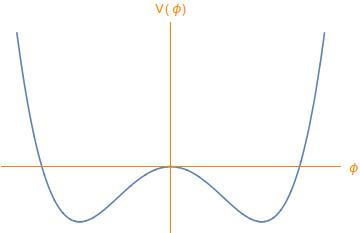
\includegraphics[width=\linewidth]{higgs}
              \caption{$\mu^{2} > 0$ için}
          \end{figure}
      \end{minipage}
      \hspace{0.05\linewidth}
      \begin{minipage}{0.45\linewidth}
          \begin{figure}[H]
              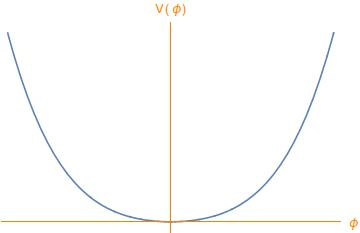
\includegraphics[width=\linewidth]{higgs2}
              \caption{$\mu^{2} < 0$ için}
          \end{figure}
      \end{minipage}
  \end{minipage}
  \caption{Potansiyel $V(\phi)$ fonksiyonu grafikleri.}
  \label{higgspot}
\end{figure}
Vakum değeri etrafında küçük pertürbasyonlar uygulamamız gerektiğinden $+v$ veya $-v$ beklenen  değerlerinden birini seçmek durumunda kalırız ve yapılan herhangi bir seçimin fiziksel sonuçları aynı olacaktır. Dolayısıyla $\phi$ alanı $\eta = \phi - v$ değeri kadar kaydırılırsa ve denklem \eqref{ksb4}'deki Lagranjiyene uygulanırsa
\begin{equation} \label{ksb7}
\begin{split}
\mathcal{L} & = \frac{1}{2} (\partial_{\mu}\eta\partial^{\mu}\eta) - \frac{1}{2}\mu_{-}^{2} \left[ \eta^{2} + 2\eta v + v^2 \right] + \frac{1}{4}\lambda \left[ \eta^{4} + 4 \eta^{3} v + 6 \eta^{2} v^{2} + 4 \eta v^{3} + v^{4 } \right] \\
 & = \frac{1}{2} (\partial_{\mu}\eta\partial^{\mu}\eta) - \lambda v^{2} \eta^{2}  + \lambda v \eta^{3} + \frac{1}{4} \lambda \eta^{4} - \frac{1}{4} \lambda v^4
\end{split}
\end{equation}
ifadesi elde edilmektedir. Buradaki $\lambda v^{2} \eta^{2}$ kütle terimi ifadesi olduğundan Klein-Gordon denkleminde belirtiğimiz üzere 
\begin{equation} \label{ksb8}
\frac{1}{2} m_{\eta}^2 = \lambda v^{2} \eta^{2} \Rightarrow m_{\eta} = \sqrt{2 \lambda v^2} \qquad \textrm{ve}\quad m_{\eta} = \sqrt{-2\mu_{-}^2} 
\end{equation}
olarak $m_{\eta}$ real ve pozitif bir kütleyi göstermektir. Lagranjiyen ifademiz her ne kadar $\phi$ yerine $\eta$ olarak temsil edilse de denklem \eqref{ksb7} ve denklem \eqref{ksb4} aynı fiziksel sistemi belirtmektedir. Dikkat çekici nokta ise Lagranjiyen ifademizde $\lambda v \eta^{3}$ olan bir terim ortaya çıktı ve bu terim nedeniyle artık Lagranjiyenimiz daha öncesinde sahip olduğu $\phi \to -\phi$ kesikli simetriye (vakum beklenen değerleri $+v$ ve $-v$ 'den başka değerler almadığı için ) $\eta \to -\eta$ olarak sahip değildir. Bu durum dışardan herhangi bir müdahele olmadan ortaya çıktığından "kendiliğinden simetri kırılması" olarak adlandırılır. 

\section{Global Simetrinin Bozulması}
Bu bölümde sürekli simetrinin bozulması incelenecektir. Öncelikle kendi kendine etkileşim halinde olan yüklü bir skaler alan için Lagranjiyen ifadesi
\begin{equation} \label{gs1}
\mathcal{L} = \left( \partial_{\mu} \phi \right)^{*} \left( \partial^{\mu} \phi \right) - V (\phi^{*}\phi) \quad \textrm{ve} \qquad \phi = \frac{\phi_{1}+i \phi_{2}}{\sqrt{2}}
\end{equation}
olarak yazılabilir. Potansiyel fonksiyonu olarak da 
$$
V(\phi^{*}\phi) = \mu^{2}(\phi^{*}\phi) + \lambda (\phi^{*}\phi)^2
$$
ifadesini aldığımızda ve $\phi = \frac{\phi_{1}+i \phi_{2}}{\sqrt{2}}$ ile belirtilen alanı Lagranjiyende yerine yazar ve düzenlersek
\begin{equation} \label{gs2}
\mathcal{L} = \frac{1}{2} \left(\partial_{\mu} \phi_{1} \right)^{2} + \frac{1}{2} \left(\partial_{\mu} \phi_{2} \right)^{2} - \frac{1}{2} \mu^{2} \left( \phi_{1}^{2} + \phi_{2}^{2} \right) - \frac{1}{4} \lambda \left( \phi_{1}^{2} + \phi_{2}^{2} \right)^{2}
\end{equation}
ifadesini elde ederiz. Bu ifade Global U(1) simetrisine sahiptir. Bunu görebilmek için $\phi^{'} \to e^{i\theta}\phi$ ve $(\phi^{*})^{'} \to e^{-i\theta}\phi^{*}$ olarak ele alındığında $\phi_{1}$ ve $\phi_{2}$ uzayında dönmeler altında değişmezdir. Bu Lagranjiyen için vakum beklenen değerleri daha önce yapıldığı üzere $\mu > 0$ ($\mu_{+}$ olarak) ve $\mu < 0$ ($\mu_{-}$ olarak) durumlarını inceleyelim. Vakum beklenen değerlerini bulabilmek için öncelikle potansiyelin minimum denklemi
\begin{equation} \label{gs3}
\begin{split}
\frac{\partial V(\phi_{1},\phi_{2})}{\partial \phi_{1}} = 0 \qquad \textrm{ve} \qquad \frac{\partial V(\phi_{1},\phi_{2})}{\partial \phi_{2}}  = 0 \\
\\
\left( \phi_{1\, min} +\phi_{2\, min} \right) \left[ \mu^{2} + \lambda \left( \phi_{1 \,min}^{2} + \phi_{2 \,min}^{2} \right) \right] = 0 
\end{split}
\end{equation}
şeklinde ifade edilir. Öncelikle $\mu_{+}$ durumunu incelediğimizda sadece $\phi_{1 \,min} = 0$ ve $ \phi_{2 \,min} = 0$ vakum beklenen değeri elde edilir. Bu nokta daha önce bahsedildiği gibi kararsız bir minimum olduğundan, Feynman cebiri uygulandığında ıraksayan ifadeler elde edilir. Dolayısıyla $\mu_{-}$ durumuna baktığımızda 
$$
\mu^{2}_{-} + \lambda \left( \phi_{1 \,min}^{2} + \phi_{2 \,min}^{2} \right) = 0 \quad \Rightarrow \quad  \sqrt{ \phi_{1 \,min}^{2} + \phi_{2 \,min}^{2} }  = \sqrt{ \frac{- \mu_{-}^{2}}{\lambda} } = v
$$
Bu çember denklemini sağlayan sonsuz sayıda $\phi_{1 \,min}$ ve $\phi_{2 \,min}$ değerleri olması sürekli bir simetriyi oluşturmaktadır. Feynman cebirini uygulayabilmek için çember üzerindeki $\phi_{1 \, min} = v$ ve $\phi_{2 \, min} = 0$ ayarlarını seçtiğimizde
$$
\eta = \phi_{1} - v \quad \textrm{ve} \quad \xi = \phi_{2} \quad \Rightarrow \quad \phi = \frac{ ( \eta + v ) + i \xi }{\sqrt{2}}
$$ 
ve Lagranjiyende yerlerine koyduğumuzda 
\begin{equation} \label{gs4}
\begin{aligned}
\mathcal{L} (\eta \,, \xi) &= \frac{1}{2} \left(\partial_{\mu} \eta \right)^{2} + \frac{1}{2} \left(\partial_{\mu} \xi \right)^{2} - \underbrace{\lambda v^{2} \eta^{2}}_{\eta\; \textrm{kütle terimi}} - \underbrace{0\, \xi^{2}}_{\xi \; \textrm{kütle terimi}} \\
\\
& - \underbrace{ \frac{1}{4} \lambda \eta^{2} - \lambda v \eta^{3} - \frac{1}{2} \lambda \eta^{2} \xi^{2} - \lambda v \eta \xi^{2} - \frac{1}{4} \lambda \xi^{4} }_{\textrm{Etkileşim terimleri}} - \underbrace{\frac{1}{4} \lambda v^{4}}_{\textrm{Sabit terim}}
\end{aligned}
\end{equation}
ifadeleri ortaya çıkmaktadır. Lagranjiyendeki $\eta$ ve $\xi$ alanlarının kütleleri olarak
\begin{equation} \label{gs5}
\frac{1}{2} m_{\eta}^{2} = \lambda v^2 \to  m_{\eta} = \sqrt{- 2 \mu^{2}_{-}} \quad m_{\eta} > 0 \quad ve \quad m_{\xi} = 0
\end{equation}
yazılabilir. Çember üzerindeki özel minimum noktaları seçtiğimizden dolayı sistemin sahip olduğu simetri bozulduğu için elde edilen Lagranjiyende $\xi$ alanı kütlesi $m_{\xi} = 0$  bir skaler alan olarak ortaya çıkmaktadır. Goldstone teoremine göre global bir simetrinin kendiğiliğinden bozulması sonucu olarak bir spin-0 kütlesiz parçacığın oluştuğunu söylemesiyle bu durumu açıklayabiliriz. Fakat bilinen parçacıkların listesinde böyle bir bozon yoktur. Dolayısla zayıf etkileşme bozonlarına kütle kazandırabilmek için teorimizde başka bir simetriyi ele almamız gereklidir.

\lhead{\emph{Abelyan Higgs Mekanizması}} 
\section{Abelyan Higgs Mekanizması}
Önceki bölümlerde yerel ayar dönüşümü altında Lagranjiyende kinetik enerji terimindeki türev işlemcisinden dolayı teorimizde foton alanı için bir kütle terimi meydana gelmişti. Teorimizi yerel ayar dönüşümü altında değişmez bırakmak istediğimizden fotonu belirten vektör alanının kütle terimini ortadan kaldırmıştık. Bu bölümde zayıf etkileşmeler için kütle terimini getirebilmek için önceki yapılanların eşliğinde bu yola başvuracağız. Lagranjiyen ifademizi
\begin{equation} \label{abe1}
\mathcal{L} = \left( \partial_{\mu} \phi \right)^{*} \left( \partial^{\mu} \phi \right) - \mu^{2}(\phi^{*}\phi) - \lambda (\phi^{*}\phi)^2 \quad \textrm{ve} \qquad \phi = \frac{\phi_{1}+i \phi_{2}}{\sqrt{2}}
\end{equation}
olarak yazalım. Yerel ayar dönüşümü için
\begin{equation} \label{abe2}
\partial_{u} \to \mathcal{D}_{\mu} = \partial_{\mu} - i \frac{q}{\hbar c} A_{\mu} \qquad \textrm{ve} \qquad A^{'}_{\mu} \to A_{\mu} + \partial_{\mu} \alpha(x)
\end{equation} 
ifadelerini kullanacağız. Burada kovaryant türev ifadesi ile eklenen  $A_{\mu} $ alanı için serbest Lagranjiyen ifadesi de eklendiğinde
$$
\mathcal{L} = \left( \mathcal{D}_{\mu} \phi \right)^{*}  \left( \mathcal{D}^{\mu} \phi \right) - \frac{1}{4} F^{\mu \nu} F_{\mu \nu} - \frac{1}{2} \mu^{2} \left( \phi_{1}^{2} + \phi_{2}^{2} \right) - \frac{1}{4} \lambda \left( \phi_{1}^{2} + \phi_{2}^{2} \right)^{2}	
$$
elde edilmektedir. Bu Lagranjiyeni daha açık bir şekilde yazarsak
\begin{equation} \label{abe3}
\begin{aligned}
\mathcal{L} &= \left[ \left( \partial_{\mu} + \frac{i\,q}{\hbar \, c} A_{\mu} \right) \left(\frac{\phi_{1} - i \phi_{2}}{\sqrt{2}} \right) \right] \left[ \left( \partial^{\mu} - \frac{i\,q}{\hbar \, c} A^{\mu} \right) \left(\frac{\phi_{1} + i \phi_{2}}{\sqrt{2}} \right) \right] \\
\\
& - \frac{1}{4} F^{\mu \nu} F_{\mu \nu} - \frac{1}{2} \mu^{2} \left( \phi_{1}^{2} + \phi_{2}^{2} \right) - \frac{1}{4} \lambda \left( \phi_{1}^{2} + \phi_{2}^{2} \right)^{2}
\end{aligned}
\end{equation}
elde edilir. Bu ifade de sadece kinetik enerji terimini düzenlediğimizde
\begin{equation} \label{abe4}
\begin{aligned}
\mathcal{L}_{Kinetik} &= \left[ \frac{1}{\sqrt{2}} \left( \partial_{\mu} \phi_{1} \right)
 - \frac{i}{\sqrt{2}} \left( \partial_{\mu} \phi_{2}  \right) + 
 \frac{i q}{\sqrt{2}\,\hbar c} \left( A_{\mu} \phi_{1} \right) +
 \frac{q }{\sqrt{2}\,\hbar c} \left( A_{\mu} \phi_{2} \right) \right] \\
 \\
 &\quad\, \left[ \frac{1}{\sqrt{2}} \left( \partial^{\mu} \phi_{1} \right)
 + \frac{i}{\sqrt{2}} \left( \partial^{\mu} \phi_{2}  \right) - 
 \frac{i q}{\sqrt{2}\,\hbar c} \left( A^{\mu} \phi_{1} \right) +
 \frac{q }{\sqrt{2}\,\hbar c} \left( A^{\mu} \phi_{2} \right) \right] \\
 \\
 &= \frac{1}{2} \left( \partial_{\mu} \phi_{1} \right)^{2} +
 \frac{1}{2} \left( \partial_{\mu} \phi_{2} \right)^{2} + 
 \frac{1}{2} \left(\frac{q}{\hbar \, c} \right)^{2} \left( \phi_{1}^{2} + \phi_{2}^{2} \right) A_{\mu} A^{\mu}\, \\
 \\
 & + \frac{q}{\hbar \, c} \bigg\lbrace  \left( \partial_{\mu}\phi_{1} \right)\phi_{2} - \left( \partial_{\mu}\phi_{2} \right) \phi_{1} \bigg\rbrace A^{\mu}
\end{aligned}
\end{equation}
olarak elde edilmektedir. Bir önceki bölümde yaptığımız gibi $\mu > 0$ ($\mu_{+}$ olarak) ve $\mu < 0$ ($\mu_{-}$ olarak) durumlarının sonuçlarını bildiğimizden vakum beklenen değeri için  $\mu_{-}$ durumunu ele alacağız ve bu bize minimumlar çemberi $$\sqrt{ \phi_{1 \,min}^{2} + \phi_{2 \,min}^{2} }  = \sqrt{ \frac{- \mu_{-}^{2}}{\lambda} } = v $$
ifadesini belirtecektir. Önceki bölümdeki gibi 
$$
\eta = \phi_{1} - v \quad \textrm{ve} \quad \xi = \phi_{2} \quad \Rightarrow \quad \phi = \frac{ ( \eta + v ) + i \xi }{\sqrt{2}}
$$ 
minimum değerleri seçildiğinde denklem \eqref{abe7}
\begin{equation*}
\begin{aligned}
\mathcal{L} &= \frac{1}{2} \left( \partial_{\mu} \eta \right)^{2} +
 \frac{1}{2} \left( \partial_{\mu} \xi \right)^{2} + 
 \frac{1}{2} \left(\frac{q}{\hbar \, c} \right)^{2} \left( (\eta + v)^{2} + \xi^{2} \right) A_{\mu} A^{\mu}\, \\
 \\
 & + \frac{q}{\hbar \, c} \bigg\lbrace  \left( \partial_{\mu} \eta  \right)\xi - \left( \partial_{\mu}\xi \right) (\eta + v) \bigg\rbrace A^{\mu}  - \lambda v^{2} \eta^{2} - 0\, \xi^{2} \\
 \\
& - \frac{1}{4} \lambda \eta^{2} -  \lambda v \eta^{3} - \frac{1}{2} \lambda \eta^{2} \xi^{2} - \lambda v \eta \xi^{2} - \frac{1}{4} \lambda \xi^{4}  - \frac{1}{4} \lambda v^{4}
 \end{aligned}
\end{equation*}
haline gelmektedir ve ifadeler düzenlendiğinde
\begin{equation} \label{abe5}
\begin{aligned}
\mathcal{L} &= \left[ \frac{1}{2} \left( \partial_{\mu} \eta \right)^{2} - \lambda v^{2} \eta^{2} \right] + 
 \left[ \frac{1}{2} \left( \partial_{\mu} \xi \right)^{2} -  0\, \xi^{2} \right]  \\
 \\
 & + \left[ - \frac{1}{4} F^{\mu \nu} F_{\mu \nu} + \frac{1}{2} \left( \frac{q}{\hbar \, c}\right)^2 v^{2} A_{\mu} A^{\mu} \right] \\  
 \\
 & + \left[ \frac{q}{\hbar \, c} \left\lbrace \left( \partial_{\mu} \eta \right) \xi - \left( \partial_{\mu} \xi \right) \eta - v \left( \partial_{\mu} \xi \right) \right\rbrace A^{\mu} \right] \\
 \\
 & + \left[ \left( \frac{q}{ \hbar \, c} \right)^{2} v \eta A_{\mu} A^{\mu} +
  \frac{1}{2} \left( \frac{q}{ \hbar \, c} \right)^{2} \left\lbrace \eta^{2} + \xi^{2} \right\rbrace A_{\mu} A^{\mu} \right] \\
  \\
 & + \left[ - \frac{1}{4} \lambda \eta^{2} -  \lambda v \eta^{3} - \frac{1}{2} \lambda \eta^{2} \xi^{2} - \lambda v \eta \xi^{2} - \frac{1}{4} \lambda \xi^{4} \right]  + \frac{1}{4} \lambda v^{4}
\end{aligned}
\end{equation}
Lagranjiyeni elde edilmektedir. Bu Lagranjiyende $\xi$ alanı kütlesiz ($m_{\xi} = 0$) spin-0 Goldstone bozonu olarak ortaya çıkmakta ve kütle kazanmış bir vektör alanı $A^{\mu}$ 
\begin{equation} \label{abe6}
\frac{1}{2}m_{A}^{2} =  \frac{1}{2} \left( \frac{q}{\hbar \, c}\right)^2 v^{2}  \quad \to \quad m_{A} = \frac{q}{\hbar \, c} v
\end{equation}
ifadesi (Proca Lagranjiyeni ifadesine benzer şekilde) meydana gelmektedir. Fakat kolayca yorumlanamaycak
$$
\frac{q}{\hbar \, c} v \, \left(\partial_{\mu}\xi \right) A^{\mu}
$$
terimi bulunmaktadır. Dolayısıyla bir şekilde $\xi$ alanında kurtulmanın yolunu bulmamız gerekir. Bunu sağlamak üzere öncelikle   vakum durumu etrafında küçük dalgalanmalar olarak betimleyebilmek için alanımızı  $\phi$'yi polar koordinatlarda
\begin{equation} \label{abe7}
\phi(x) = \frac{1}{\sqrt{2}} \left( \eta (x) + v \right) e^{i \frac{\xi (x)}{v}}
\end{equation}
olarak yazarız. Burada yerel olarak bir ayar dönüşümü yaparak $\phi$ alanının fazını sadece real kısımı kalacak şekilde $\xi$ alanını ortadan kaldırabiliriz. Bunu yapabilmek için $\alpha(x) = - \frac{\xi (x)}{v} $ olarak adlandıralan birimsel ayarı seçeriz ve buna bağlı olarak yerel ayar dönüşümü $\phi(x)$ alanı için
\begin{equation} \label{abe8}
\begin{aligned}
\left(\phi(x)\right)^{'} &\xrightarrow{U(1)}   e^{-i \frac{\xi (x)}{v}} \phi(x) \\
\\
& \xrightarrow{U(1)} e^{-i \frac{\xi (x)}{v}} \frac{1}{\sqrt{2}} \left( \eta (x) + v \right) e^{i \frac{\xi (x)}{v}} \\
\\
& \xrightarrow{U(1)} \frac{1}{\sqrt{2}} \left( \eta (x) + v \right) = \frac{1}{\sqrt{2}} \left( H(x) + v \right)
\end{aligned}
\end{equation}
ifadesini elde ederiz. Görüldüğü üzere bu dönüşüm sonucu $\xi$ alanında kurtulmuş olduk. $A_{\mu}$ alanı da
\begin{equation} \label{abe9}
\begin{aligned}
&A^{'}_{\mu} \xrightarrow{U(1)} A_{\mu} - \frac{1}{q v}(\partial_{\mu} \xi)\,, \qquad\quad B_{\mu} \equiv A_{\mu} - \frac{1}{q v}(\partial_{\mu} \xi) \\
\\
& F^{\mu \nu} \xrightarrow{U(1)} \left( \partial^{\mu} A^{\nu} - \partial^{\nu} A^{\mu} \right)^{'} \equiv \partial^{\mu} B^{\nu} - \partial^{\nu} B^{\mu} \equiv F^{\mu \nu}(B)
\end{aligned}
\end{equation}
olarak dönüşmektedir. Bu değişiklikleri gerçekleştirdikten sonra Lagranjiyen ifademizi tekrar yazarsak
\begin{equation*}
\begin{aligned}
\mathcal{L} &= \left( \mathcal{D}_{\mu} \phi)^{*} (\mathcal{D}^{\mu} \phi \right) - \frac{1}{4} F^{\mu \nu} F_{\mu \nu} - \mu_{-}^{2}(\phi^{*} \phi) - \lambda (\phi^{*} \phi)^{2}\\
\\
& = \left[ \left( \partial_{\mu} + \frac{i\,q}{\hbar \, c} B_{\mu} \right) \left( \frac{\left( H(x) + v \right)}{\sqrt{2}} \right) \right] \left[ \left( \partial^{\mu} - \frac{i\,q}{\hbar \, c} A^{\mu} \right) \left( \frac{\left( H(x) + v \right)}{\sqrt{2}} \right) \right] \\
\\ 
& - \frac{1}{4} F^{\mu \nu}(B) F_{\mu \nu}(B) - \mu_{-}^{2} \left( \frac{\left( H(x) + v \right)}{\sqrt{2}} \right)^{2} - \lambda \left( \frac{\left( H(x) + v \right)}{\sqrt{2}} \right)^{4}\\
\\
\end{aligned}
\end{equation*}
ve düzenlersek
\begin{equation} \label{abe10}
\begin{aligned}
\mathcal{L} &= \underbrace{ \left[ \frac{1}{2} \left( \partial_{\mu} H \right) - \lambda v^2 H^2 \right] }_{\textrm{ Kütleli H(x) skaler alanı}} +
 \underbrace{ \left[ - \frac{1}{4} F^{\mu \nu}(B) F_{\mu \nu}(B) +  \frac{1}{2} \left( \frac{q}{\hbar \,c} \right)^{2} v^2 B_{\mu} B^{\mu} \right] }_{ \textrm{Kütleli } B_{\mu} \textrm{ vektör alanı} } \\
\\
& + \underbrace{ \left[ \frac{1}{2} \left( \frac{q}{\hbar \,c} \right)^{2} H^2 B_{\mu} B^{\mu} + \left( \frac{q}{\hbar \,c} \right)^{2} H\, v B_{\mu} B^{\mu} \right] }_{ \textrm{H(x) alanı ve } B_{\mu} \textrm{ etkileşim terimi}} \\
\\
& - \underbrace{\left[ \lambda \, v  H^{3} + \frac{1}{4} \lambda H^{4} \right]}_{\textrm{H(x) alanı kendisiyle etkileşimi}} + \underbrace{\frac{1}{4} \lambda v^4}_{\textrm{Sabit terim}}
\end{aligned}
\end{equation} 
elde edilir. Buradaki H(x) alanı Higgs kütleli skaler alanını temsil etmektedir. Görüldüğü üzere artık kütle kazanmış bir $B_{\mu}$ vektör alanı ve fiziksel gerçeği temsil etmeyen kütlesiz Goldstone bozonu ayrıca diğer terimlerden de kurtulmuş olduk. Denklem \eqref{abe10}'daki ifadenin kendiliğinden simetri bozulmasına uğramadan önce polarizasyon sayısı
$$
\left(2 A_{\mu}\right) + 2 \left( \phi \right) = 4 \
$$
ve kendiliğinden simetri bozulmasına uğradıktan sonra polarizasyon sayısı
$$
\left(3 B_{\mu}\right) + 1 \left( H \right) = 4
$$
olmak üzere toplam serbestlik derecesi değişmeden kalmaktadır. $A_{\mu}$ kütlesiz vektör alanının enine kutuplanmalar olmak üzere iki serbestlik derecesi vardır. Artık kütle kazanmış $B_{\mu}$ alanını iki adet enine kutuplanması olmasının yanında bir de boyuna kutuplanma serbestlik derecesine sahip olmaktadır. Ayrıca Lagranjiyende kütleli ayar teorisinin renormalize edilebilirliği de korunmaktadır. Higgs mekanizması zorunlu olarak bir Higgs parçacığının var olması gerektiğini ima etmemektedir. Fakat polarizasyon derecesinin korunması böyle bir parçacığı da ortaya çıkmaktadır. Lagrenjiyendeki kütle terimlerinden
\begin{equation} \label{abe11}
\begin{aligned} 
&\frac{1}{2} m_{H}^{2} = \lambda v^2 \quad \Rightarrow \quad m_{H} = \sqrt{2 \lambda v^2} = \sqrt{- 2 \mu_{-}} \quad m_{H} > 0 \\
\\
& \frac{1}{2} m_{B}^{2} = \frac{1}{2} \left( \frac{q}{\hbar \,c} \right)^{2} v^2 \quad \Rightarrow \quad m_{B} = \frac{q}{\hbar \,c} v \quad m_{B} > 0
\end{aligned}
\end{equation}
ifadeleri ile  bulunur. Higgs'in kütlesi $\lambda$ olan bilinmeyen bir parametreye bağlıdır. Dolayısıyla Higgs'in kütlesinin önceden belirlenmesine engel olan bir durum açığa çıkmaktadır. Higgs alanının önemli bir diğer özelliği de vakum beklenen değeri sıfır olmayan spin-0 bir skaler alan olmasıdır. Dolayısıyla uzayın her tarafında değeri sıfır olmayan bir alanın varlığını göstermektedir.

%\lhead{\emph{Abelyan Higgs Mekanizması}} 
\section{Standart Modelde Higgs Mekanizması}

 % Background Theory 

\chapter{Standart Model Higgs Bozonunun Araştırılması}

\section{Higgs Bozonu Özellikleri}

\section{Higgs Bozonunun Üretimi}

\section{Higgs Bozonunun Bozunumu}
 % Experiment 1

%\input{Chapters/Chapter5} % Experiment 2

%\input{Chapters/Chapter6} % Results and Discussion

%\input{Chapters/Chapter7} % Conclusion

%% ----------------------------------------------------------------
% Now begin the Appendices, including them as separate files

\addtocontents{toc}{\vspace{2em}} % Add a gap in the Contents, for aesthetics

\appendix % Cue to tell LaTeX that the following 'chapters' are Appendices

\chapter{An Appendix}

Lorem ipsum dolor sit amet, consectetur adipiscing elit. Vivamus at pulvinar nisi. Phasellus hendrerit, diam placerat interdum iaculis, mauris justo cursus risus, in viverra purus eros at ligula. Ut metus justo, consequat a tristique posuere, laoreet nec nibh. Etiam et scelerisque mauris. Phasellus vel massa magna. Ut non neque id tortor pharetra bibendum vitae sit amet nisi. Duis nec quam quam, sed euismod justo. Pellentesque eu tellus vitae ante tempus malesuada. Nunc accumsan, quam in congue consequat, lectus lectus dapibus erat, id aliquet urna neque at massa. Nulla facilisi. Morbi ullamcorper eleifend posuere. Donec libero leo, faucibus nec bibendum at, mattis et urna. Proin consectetur, nunc ut imperdiet lobortis, magna neque tincidunt lectus, id iaculis nisi justo id nibh. Pellentesque vel sem in erat vulputate faucibus molestie ut lorem.

Quisque tristique urna in lorem laoreet at laoreet quam congue. Donec dolor turpis, blandit non imperdiet aliquet, blandit et felis. In lorem nisi, pretium sit amet vestibulum sed, tempus et sem. Proin non ante turpis. Nulla imperdiet fringilla convallis. Vivamus vel bibendum nisl. Pellentesque justo lectus, molestie vel luctus sed, lobortis in libero. Nulla facilisi. Aliquam erat volutpat. Suspendisse vitae nunc nunc. Sed aliquet est suscipit sapien rhoncus non adipiscing nibh consequat. Aliquam metus urna, faucibus eu vulputate non, luctus eu justo.

Donec urna leo, vulputate vitae porta eu, vehicula blandit libero. Phasellus eget massa et leo condimentum mollis. Nullam molestie, justo at pellentesque vulputate, sapien velit ornare diam, nec gravida lacus augue non diam. Integer mattis lacus id libero ultrices sit amet mollis neque molestie. Integer ut leo eget mi volutpat congue. Vivamus sodales, turpis id venenatis placerat, tellus purus adipiscing magna, eu aliquam nibh dolor id nibh. Pellentesque habitant morbi tristique senectus et netus et malesuada fames ac turpis egestas. Sed cursus convallis quam nec vehicula. Sed vulputate neque eget odio fringilla ac sodales urna feugiat.

Phasellus nisi quam, volutpat non ullamcorper eget, congue fringilla leo. Cras et erat et nibh placerat commodo id ornare est. Nulla facilisi. Aenean pulvinar scelerisque eros eget interdum. Nunc pulvinar magna ut felis varius in hendrerit dolor accumsan. Nunc pellentesque magna quis magna bibendum non laoreet erat tincidunt. Nulla facilisi.

Duis eget massa sem, gravida interdum ipsum. Nulla nunc nisl, hendrerit sit amet commodo vel, varius id tellus. Lorem ipsum dolor sit amet, consectetur adipiscing elit. Nunc ac dolor est. Suspendisse ultrices tincidunt metus eget accumsan. Nullam facilisis, justo vitae convallis sollicitudin, eros augue malesuada metus, nec sagittis diam nibh ut sapien. Duis blandit lectus vitae lorem aliquam nec euismod nisi volutpat. Vestibulum ornare dictum tortor, at faucibus justo tempor non. Nulla facilisi. Cras non massa nunc, eget euismod purus. Nunc metus ipsum, euismod a consectetur vel, hendrerit nec nunc.	% Appendix Title

%\input{Appendices/AppendixB} % Appendix Title

%\input{Appendices/AppendixC} % Appendix Title

\addtocontents{toc}{\vspace{2em}}  % Add a gap in the Contents, for aesthetics
\backmatter

%% ----------------------------------------------------------------
\label{Bibliography}
\lhead{\emph{Bibliography}}  % Change the left side page header to "Bibliography"
\bibliographystyle{unsrtnat}  % Use the "unsrtnat" BibTeX style for formatting the Bibliography
\bibliography{Bibliography}  % The references (bibliography) information are stored in the file named "Bibliography.bib"

\end{document}  % The End
%% ----------------------------------------------------------------